
\section{Numerical Experiments}
This section is organized as follows. The first part is dedicated to the numerical implementation
of the frequency domain formulation (\ref{eq:main_frequency_domain}). We study the convergence of this formulation and the behaviour 
of the numerical solution as the absorption parameter $\nu$ tends to zero. The experiments in this section were 
performed on a laptop with 2.6GHz Intel Core i5 CPU, with the help of the code written in Octave (compatible with Matlab). 
We implemented the scheme described in Section \ref{sec:discr} for a simple case of $P_{1}$-space used 
for the approximation of $E_{x}$ and $E_{y}$ and $\theta=0$, thus working with the system (\ref{eq:simple_system}). 
We apply permutation to the above system 
to obtain a 7-diagonal Hermitian matrix and solve the system with the Gauss back substitution algorithm. 

The second part of the section deals with the question of the equivalence of the limiting absorption and limited amplitude 
principle. We compare the solutions obtained as $\nu\rightarrow 0$ with the help of our frequency domain code 
and of the time domain code (computed for large values of time). 
The time-domain code implements the scheme described in Section \ref{sec:discr} and 
is written in Fortran. 
\subsection{Frequency Domain Problem}
\label{sec:freq_dep}
\subsubsection{Validity of Implementation}
To check the validity of the code, we perform a numerical experiment with (formally chosen) parameters:
\begin{align}
\label{eq:parameters}
\alpha(x)=x^2+1,\qquad \delta(x)=\left(\alpha^2+x\alpha\right)^{\frac{1}{2}}.
\end{align}
Additionally, the boundary conditions read as 
\bealn
\label{eq:bcs}
\partial_{1}E_{y}(-L)+2iE_{y}(-L)=2iAi(-L)+Ai'(-L),\\
\partial_{1}E_{y}(H)=0,
\eealn
where $Ai(x)$ is the Airy function. 
For more detail on Airy functions and the Airy equation see \cite[Chapter 10.4]{abramowitz_stegun}.

It can be shown that $E_{y}$ thus satisfies the Airy equation, and hence, 
with the choice of the boundary conditions as above, we obtain that 
\bealn
E_{y}=Ai(x),\qquad 
E_{x}=-i\frac{\delta(x)}{\alpha(x)}Ai(x)
\ealn
is the solution to the problem with parameters (\ref{eq:parameters}) with the boundary condition (\ref{eq:bcs}).

In Fig.~\ref{fig:conv_rate} we demonstrate the convergence rates for this problem, with 
\ben
\|E_{x}-E_{x}^{c}\|_{L_{2}(\Omega)}=\left(\int\limits_{\Omega}\left|E_{x}(x)-\sum\limits_{k=1}^{N}e_{xk}\phi_{k}\right|^2dx\right),
\een
where $\left(\phi_{i}\right)_{i=1}^{N}$ are $P_{1}$-finite elements and $E_{x}(x)$ is a known analytic solution. Similarly $\|E_{y}-E_{y}^{c}\|_{L_{2}(\Omega)}$ and $\|E_{y}-E_{y}^{c}\|_{H_{1}(\Omega)}$ are defined. 

\begin{figure}
\begin{tikzpicture}
    \begin{loglogaxis}[
        xlabel=$h$,
        ylabel=$Error$,
        width=0.4\textwidth,
        legend style={
at={(1.7,0.5)},
%legend pos=outer north east, 
anchor=east,
%legend pos=south east,
%anchor=east, 
draw=none,
font=\small
}
]\addplot[mark=*,blue] table {pics/E1L2.dat}; 
    \addlegendentry{$\|E_{x}-E_{x}^{c}\|_{L_{2}}$};
    \addplot[mark=*,red] table {pics/E2H1.dat};
        \addlegendentry{$\|E_{y}-E_{y}^{c}\|_{H_{1}}$};
        
          \addplot[mark=*,cyan] table {pics/E2L2.dat};
        \addlegendentry{$\|E_{y}-E_{y}^{c}\|_{L_{2}}$};  
        \addplot[dotted] table{pics/E_h2.dat};
         \addlegendentry{$O(h^2)$};
         \addplot[dashed] table{pics/H.dat};
         \addlegendentry{$O(h)$};
    \end{loglogaxis}
    \end{tikzpicture}
    \caption{Convergence rates for the problem with parameters (\ref{eq:parameters}) with the boundary condition (\ref{eq:bcs}).}
    \label{fig:conv_rate}
\end{figure}

Note that in the last 3 experiments the error of the solution of the system of equations, namely $\|Ae-r\|$ (where $e$ is the solution vector, $r$ is the right hand side and $A$ is the block matrix (\ref{eq:simple_system}) ) exceeded 1.6e-9
(namely, it was 1.6e-9 ($h=3.2e-5$), 1.3e-08 ($h=8e-6$), 1.04e-07 ($h=2e-6$)).

Importantly, the obtained convergence rates are in agreement with known estimates of \cite{brenner}.



\subsubsection{Solution of $X$-Mode Prolbem}
\paragraph{Convergence}
Let us consider the case of the resonance, more precisely, we consider sufficiently smooth
$\alpha,\delta$, s.t. $\alpha(0)=0$ and $\delta(0)\neq 0$, and the solvability conditions 
of Lemma \ref{lemma:well_posedness}  are satisfied. 
For simplicity, let us consider 
\begin{align}
\label{eq:cond}
 \alpha(x)=-x \text{  in some neighbourhood of $0$ }.
\end{align}
Given $\mathbf{V}_{h}=P_{h}^{1}\times P_{h}^{1}$, with $P_{h}^{1}$ consisting of piecewise-linear (hat) functions, 
we look for a ratio $h(\nu)$ that would ensure that the absolute error 
\begin{align}
\label{eq:problem1}
\|E^{\nu}_{x}-E^{\nu,h}_{x}\|_{L_{2}(\Omega)}<\epsilon,
\end{align}
given a fixed value of $\epsilon>0$. 

We use the following well-known facts:
\begin{itemize}
 \item The C\'ea's lemma applied to the problem (\ref{vf1dcase}); here $C_c$ is the continuity and $C_i$ is the coercivity constants:
\begin{align}
\label{eq:cea}
\begin{split}
 \|\mathbf{E}^{\nu}-\mathbf{E}^{h,\nu}\|_{V}\leq \frac{C_c}{C_i}\min_{\mathbf{v}\in V_h}\|\mathbf{E}-\mathbf{v}\|_{V}
 \leq \nu^{-1}\min_{\mathbf{v}\in V_h}\|\mathbf{E}-\mathbf{v}\|_{V}.
 \end{split}
\end{align}
The last inequality follows from Lemma \ref{lemma:well_posedness}.  
\item The form of the exact solution to the problem (\ref{vf1dcase}):
\begin{align}
\label{eq:exact}
 E_x^{\nu}=E_{y}^{\nu}\frac{\delta}{\alpha+i\nu}=\frac{f(x)}{\alpha(x)+i\nu},
\end{align}
for some $f(x)\in L_{2}(\Omega)$. 
\item The estimate from \cite[Chapter 0]{brenner} on the rate of convergence of the interpolation 
\begin{align}
\label{eq:bsc}
 \|v-I^{h}v\|_{L_{2}(\Omega)}\leq Ch^2|v''|_{L_{2}(\Omega)},\; C>0,
 %\\ \|v-I^{h}v\|_{H_{1}(\Omega)}\leq Ch|v''|_{L_{2}(\Omega)},\; C>0, 
\end{align}
where $I^{h}v$ is an interpolation operator onto $P_{h}^{1}$.
\end{itemize}
For $E_x^{\nu},\;f(x)$ in (\ref{eq:exact}) being sufficiently smooth, 
\ben
 \frac{d^2}{dx^2}E_x^{\nu}=\frac{f''}{\alpha+i\nu}-2\frac{f'\alpha'}{(\alpha+i\nu)^2}+\frac{f\alpha''}{(\alpha+i\nu)^3},
\een
from which, together with (\ref{eq:cond}), it follows that there exists $c>0$ s.t. for all sufficiently small $\nu$ 
\ben
 \left|  \frac{d^2}{dx^2}E_x^{\nu}\right|_{L_2}^{2}&\leq c\int\limits_{\Omega}\frac{1}{(x^2+\nu^2)^{3}}dx
 %\\
 %&=c\left.
 %\left(\frac{x}{4(x^2+\nu^2)^2}\nu^{-2}+\frac{3x}{8(x^2+\nu^2)}\nu^{-4}+\frac{3}{8}\nu^{-5}\operatorname{atan}\frac{x}{\nu}\right)\right|_{-L}^{H}
 \leq C\nu^{-5},\; 
\een
where $C>0$ does not depend on $\nu$. This, together with the estimates (\ref{eq:cea}) and (\ref{eq:bsc}), results in 
\ben
 \|E^{\nu}_{x}-E^{\nu,h}_{x}\|_{L_{2}(\Omega)}\leq C\nu^{-\frac{7}{2}}h^2,
\een
from which it follows that to ensure (\ref{eq:problem1}) $h$ should be chosen as 
\begin{align}
\label{eq:estimate_h}
 h=\alpha_{\epsilon}\nu^{\frac{7}{4}},
\end{align}
where $\alpha_{\epsilon}>0$ depends on $\epsilon$ but does not depend on $\nu$. 

Let us check whether this holds true. 
To do so, we conduct the  numerical experiment with parameters for the problem as given in Table \ref{tab:parameters}.
\begin{table}
\begin{tabular}{l|r}
Parameter & Value \\
\hline
$\alpha(x)$ & $\left\{\begin{array}{cc}
10, & x\leq -10,\\
-x, & -10<x\leq 5,\\
-5, & x>5.
\end{array}\right.$ \\
$\delta(x)$ & 
$\left\{\begin{array}{cc}
0, & x\leq -10,\\
4/30x+4/3,& -10<x\leq 5,\\
2, & x>5.
\end{array}\right.$ \\
$g^{inc}(-L)$ & $-2 \sqrt{2}i\exp(-22\sqrt{2}i)$\\
$\lambda$ & 
$\sqrt{10}$\\
$L$& 15\\
$H$ & 10 \\
\end{tabular}
\caption{The parameters for the problem with the resonance}
\label{tab:parameters}
\end{table}

 We fix $\nu$ and compute the error of the solution compared to the solution computed on the finest mesh  (with $h=2e-6$). 
 The results are depicted in Fig. \ref{fig:dependence} and \ref{fig:l2_err_e2}.
\begin{figure}
\begin{tabular}{cc}
\begin{tikzpicture}
    \begin{loglogaxis}[
    	width=0.5\textwidth,
    	height=0.5\textwidth,
        xlabel=$h$,
        ylabel=$Error$,
        legend style={
at={(0.2,1.5)},
legend pos= south east,
anchor=south east, 
draw=none, 
font=\tiny
}
]
\addplot[mark=*,blue] table {pics/result_l2e1.1.dat}; 
\addlegendentry{$\nu=1$};
\addplot[mark=*,green] table {pics/result_l2e1.0.25.dat}; 
\addlegendentry{$\nu=2^{-2}$};
\addplot[mark=*,red] table {pics/result_l2e1.0.0625.dat}; 
\addlegendentry{$\nu=2^{-4}$};
\addplot[mark=square,blue] table {pics/result_l2e1.0.015625.dat}; 
\addlegendentry{$\nu=2^{-6}$};
\addplot[mark=square,green] table {pics/result_l2e1.0.0039062.dat}; 
\addlegendentry{$\nu=2^{-8}$};
\addplot[mark=triangle,red] table {pics/result_l2e1.0.00097656.dat}; 
\addlegendentry{$\nu=2^{-10}$};
\addplot[mark=triangle,blue] table {pics/result_l2e1.0.00024414.dat}; 
\addlegendentry{$\nu=2^{-12}$};
\addplot[mark=triangle, green] table {pics/result_l2e1.6.1035e-05.dat};
\addlegendentry{$\nu=2^{-14}$};
\addplot[mark=triangle, red] table{pics/result_l2e1.1.5259e-05.dat};
\addlegendentry{$\nu=2^{-16}$};
\end{loglogaxis}
\end{tikzpicture} &
\begin{tikzpicture}
    \begin{loglogaxis}[
    	width=0.5\textwidth,
    	height=0.5\textwidth,
        xlabel=$h$,
        ylabel=$Error$,
        ymin=1e-8,
        legend style={
at={(0.2,1.5)},
legend pos= south east,
anchor=south east, 
draw=none,
font=\tiny
}
]
\addplot[mark=*,blue] table {pics/result_l2e2.1.dat}; 
\addlegendentry{$\nu=1$};
\addplot[mark=*,green] table {pics/result_l2e2.0.25.dat}; 
\addlegendentry{$\nu=2^{-2}$};
\addplot[mark=*,red] table {pics/result_l2e2.0.0625.dat}; 
\addlegendentry{$\nu=2^{-4}$};
\addplot[mark=square,blue] table {pics/result_l2e2.0.015625.dat}; 
\addlegendentry{$\nu=2^{-6}$};
\addplot[mark=square,green] table {pics/result_l2e2.0.0039062.dat}; 
\addlegendentry{$\nu=2^{-8}$};
\addplot[mark=square, red] table {pics/result_l2e2.0.00097656.dat}; 
\addlegendentry{$\nu=2^{-10}$};
\addplot[mark=triangle,blue] table {pics/result_l2e2.0.00024414.dat}; 
\addlegendentry{$\nu=2^{-12}$};
\addplot[mark=triangle, green] table{pics/result_l2e2.6.1035e-05.dat};
\addlegendentry{$\nu=2^{-14}$};
\addplot[mark=triangle, red] table{pics/result_l2e2.1.5259e-05.dat};
\addlegendentry{$\nu=2^{-16}$};
\end{loglogaxis}
\end{tikzpicture} 
\end{tabular}
\caption{In the left figure we show the $L_{2}$-error of $E_{x}(x)$, and in the right figure the $L_2$-error of $E_y(x)$ is shown.}
\label{fig:l2_err_e2}
\end{figure} 

Let us denote by $E_{x}^{h}$ the solution $E_{x}(x)$ computed on the mesh with a width $h$, and by $E_{x}^{c}$ the solution computed on the finest mesh. We introduce 
\begin{align}
\label{eq:def_epsilon}
h_{\epsilon}=\sup\{h: \|E_{x}^{h'}-E_{x}^{c}\|<\epsilon \text{ for all } h'<h\}.
\end{align}
The computed dependence of $h_{\epsilon}$ on $\nu$ is shown in Fig.~\ref{fig:dependence}.
\begin{figure}
\begin{tabular}{cc}
\begin{tikzpicture}
    \begin{loglogaxis}[
    	width=0.5\textwidth,
    	height=0.5\textwidth,
        xlabel=$\nu$,
        ylabel=$h_{\epsilon}$,
        legend style={
at={(0.2,1.5)},
legend pos= south east,
anchor=south east, 
draw=none
}
]
\addplot[mark=*,blue] table {pics/h1e-1.dat}; 
\addlegendentry{$\epsilon=1e-1$};
%\addplot[mark=o,red] table {pics/h1e-2.dat}; 
%\addlegendentry{$\epsilon=1e-2$};
\addplot[mark=triangle,green] table {pics/h1e-3.dat}; 
\addlegendentry{$\epsilon=1e-3$};
%\addplot[mark=square,cyan] table {pics/h1e-4.dat}; 
%\addlegendentry{$\epsilon=1e-4$};
\addplot[dashed, red] table {pics/nu1.dat}; 
\addlegendentry{$O(\nu)$};
\addplot[dashed, blue] table {pics/nu32.dat}; 
\addlegendentry{$O(\nu^{\frac{3}{2}})$};
\end{loglogaxis}
\end{tikzpicture} 
&
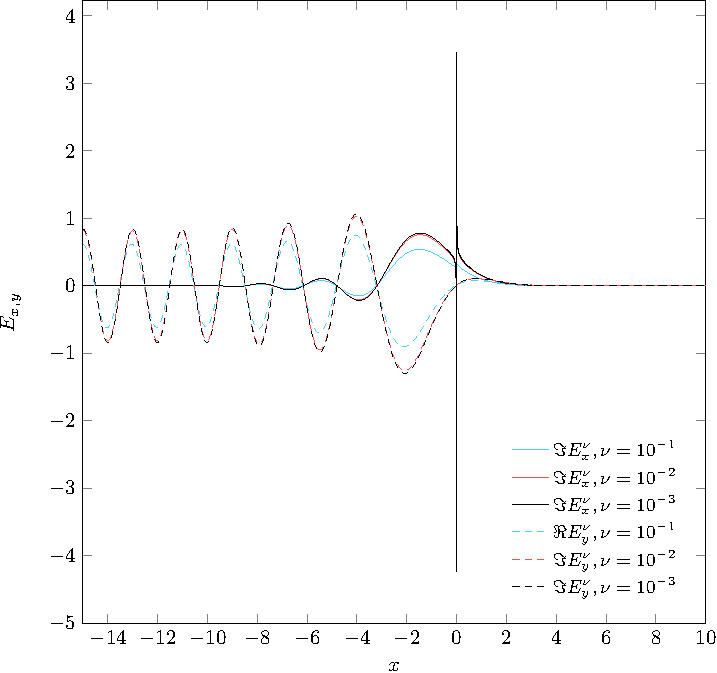
\includegraphics[width=0.5\textwidth]{figure1-crop.pdf}
\end{tabular}
\caption{In the left figure the depenence of $h_{\epsilon}$ as defined by (\ref{eq:def_epsilon}) on $\nu$ is demonstrated. 
In the right figure we show the solutions for the problem for different values of $\nu$. }
\label{fig:dependence}
\end{figure}

We can see that the estimate (\ref{eq:estimate_h}) is pessimistic compared to the one suggested by (\ref{eq:def_epsilon}), 
at least for a given value of $\epsilon$.


\begin{remark}
 We can show that 
\bealn
 \|E^{\nu}_{x}\|_{L_{2}(\Omega)}\leq \frac{C}{\sqrt{\nu}},\; C>0, 
\eealn
and thus the relative error control
\bealn
 \frac{\|E^{\nu}_{x}-E^{\nu,h}_{x}\|_{L_{2}(\Omega)}}{\|E^{\nu}_{x}\|_{L_{2}(\Omega)}}\leq \epsilon
\eealn
can be ensured by choosing $h$ as $\beta_{\epsilon}\nu^{\frac{3}{4}}$.
\end{remark}

\FloatBarrier
\paragraph{Condition Number}

We consider the dependence of the condition number of the matrix of the system (\ref{eq:simple_system}) 
on $\nu$, for several values of $h$ (see Table \ref{tab:cond_number}).
\begin{table}[ht!]
\begin{tabular}{c|ccccccccc}
\diagbox[width=10em]{$h$}{$\nu$}& 100 & 10 & 1 & 0.1 & 1e-2 & 1e-3 & 1e-4 & 1e-8 & 0\\
 \hline
1 & 3.9634&4.3787 &4.987&36.949&42.394& 42.757 &42.79&42.793&42.793\\
\hline
0.5&      3.9931& 6.87&48.473 & 168.41  &207.34  & 209.63 & 209.83 & 209.85&  209.85\\
\hline
 0.1&      16.09  &     159.56  &     1146.1   &    8304.1   &     19169  &      20270   &     20344   &     20352   &     20352\\
 \hline
0.05&      64.046  &     637.18  &     4686.2   &     38876 &  1.4e5 &  1.58e5 &   1.58e5 &  1.58e5 &  1.58e5\\
\hline
 0.01&       1600    &   15921 & 1.2e5  & 1.1e6 & 8.3e6  & 1.8e7   & 1.93e7  & 1.93e7  & 1.93e7\\
\end{tabular}
\caption{The condition number of the matrix of the system (\ref{eq:simple_system}) for different values of $\nu$ and $h$. }
\label{tab:cond_number}
\end{table}
Remarkably, for $\nu=0$ the computed matrices are not singular. \urev{We do not know the exact reason for such a behavior.}
As an additional illustration, we compare the solutions for very small $\nu$ and $\nu=0$ for different meshes in Fig.~\ref{fig:small_nu}. 
\begin{figure}
 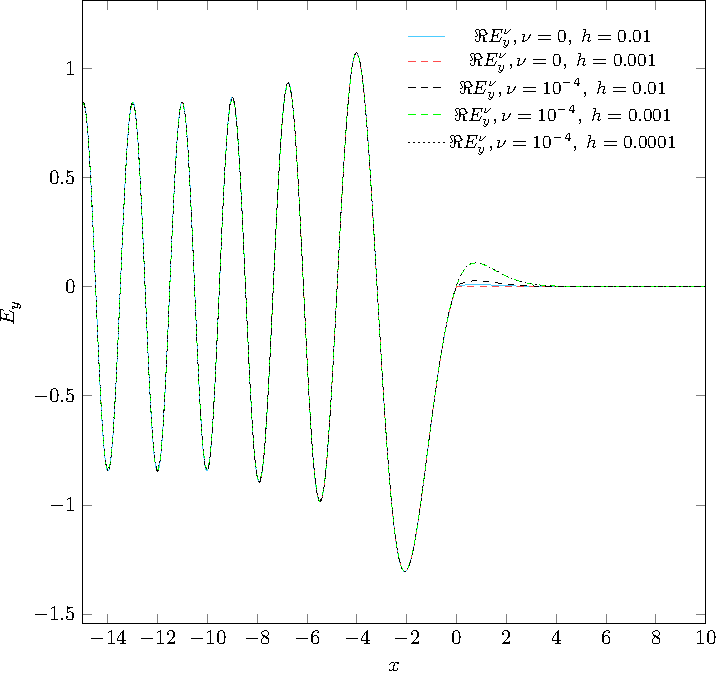
\includegraphics[width=0.4\textwidth]{figure2-crop.pdf}
 \caption{The plot shows $E_{y}^{\nu}$ computed on different meshes for small $\nu$. It can be seen that for meshes that are coarse 
 with respect to $\nu$ (e.g. $\nu=10^{-4}, \; h=10^{-2}$, or $\nu=0,\; h=10^{-2}$), the computed solution seems to be only piecewise-continuous in $\nu$, 
 while for finer meshes and $\nu>0$ the solution seems to be smooth. It can be also seen that for $h=10^{-2}$ and $h=10^{-3}$ the solutions 
 computed for $\nu=0$ are indistinguishable on this scale.}
 \label{fig:small_nu}
\end{figure}




%\subsubsection{No-Resonance Case}
%We choose the parameters so that in the frequency domain, for the limiting amplitude problem, $\hat{E}_{2}$ satisfies 
%the Airy equation \cite{}. 

%We set $\omega_c=0$ (thus $\delta(x)=0$), $\omega=1$ (hence $\alpha(x)=1-N_e(x)$), 
%choose the domain as $[-0.5, 10]$ and set the electron density $N_e(x)=1+x$. Importantly, $N_e(x)>0$ on the whole interval.
%The boundary conditions in (\ref{eq:bcs}) are chosen as $G=Ai'(0.5)$. 
%In all the experiments in this section the CFL number was chosen to be equal to 0.5.


%First let us fix $\nu=1e-2$. 
%To demonstrate that the limiting amplitude principle indeed holds, we fix a point $x=x_c$ 
%inside the domain $(-L,\; H)$ and plot the dependence of the solution $E_{y}^{\nu}(x_c,t), \; \hat{E}_2^{\nu}(x_c)\mathrm{e}^{it}$ 
%on time $t$ for a range of $t\gg 1$ in Figure \ref{fig:nu1e2_harmon}.  